\documentclass[a4paper, 11pt]{article}
\usepackage[czech]{babel}
\usepackage[utf8]{inputenc}
\usepackage[text={17cm, 24cm}, lmargin=2cm, tmargin=3cm]{geometry}
\bibliographystyle{czplain}
\usepackage{url}
\usepackage{listings}
\usepackage{graphicx}
\DeclareUrlCommand\url{\def\UrlLeft{<}\def\UrlRight{>} \urlstyle{tt}}

\begin{document}
    \begin{titlepage}
        \begin{center}
            \textsc{\Huge Vysoké učení technické v~Brně}\\[0.6em]
            \textsc{\huge Fakulta informačních technologií}\\
            \vspace{\stretch{0.382}}
            {\LARGE Dokumentace k projektu} \\[0.3em] {\Huge Export DNS informací pomocí protokolu Syslog}\\
            \vspace{\stretch{0.618}}
        \end{center}
        {\Large \today \hfill
        Petr Šopf (xsopfp00)}
    \end{titlepage}
    
 
\newpage
  \tableofcontents
\newpage

\section{Implementace}
Tato sekce obsahuje popis implementace jednotlivých částí programu. Obsahuje také výpis potřebných teoretických znalostí.

\subsection{Zpracovávání packetů}
Zpracovávání packetů probíhá za pomocí knihovny \verb|libpcap|. Veškeré informace jsem čerpal z oficiální dokumentace této knihovny \cite{tcpdump:dokumentace}. Nejprve dochází k volání funkcí \verb|pcap_open_offline| v případě čtení z~pcap souboru a \verb|pcap_open_live| v případě naslouchání na síťovém rozhraní. Následně je kompilován a nastaven filtr na port 53, tedy na port pro DNS komunikaci. Nakonce dojde k volání funkce \verb|pcap_loop|, která zajistí zpracování všech DNS packetů. Tato funkce volá jako callback další funkci, která již zpracovává packet jako takový.

Nejprve dojde ke zpracování ethernetové hlavičky a určení, jestli se jedná o protokol IPv4 nebo IPv6. Zatímco hlavička IPv6 má konstantní velikost 40 bytů \cite{Wikipedie:IPv6}, tak velikost hlavičky IPv4 je nutné vypočítat \cite{Wikipedie:IPv4}. V hlavičce těchto protokolů také nalezneme informaci o použitém protokolu transportní vrstvy.

Následně dojde k určení a zpracování protokolu transportní vrstvy. V případě UDP je vše jednoduché, jelikož hlavička UDP protokolu je konstantní a to 8 bytů. Velikost TCP hlavičky je pak nutné vypočítat \cite{Firewall:tcp}.

Po protokolu transportní vrstvy už konečně následuje protokol DNS. Struktura DNS packetu je následující:

\begin{center}
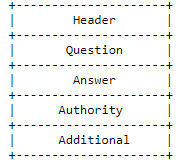
\includegraphics[width=0.2\textwidth]{img/dns-struct.png}
\end{center}

Nejprve je tedy nutné zpracovat hlavičku, která má následující strukturu:

\begin{center}
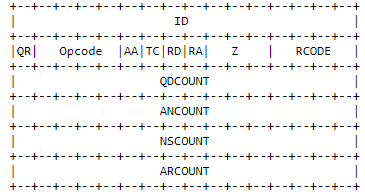
\includegraphics[width=0.4\textwidth]{img/dns-header-struct.png}
\end{center}

Nejdůležitějším údajem je pro nás hodnota \textbf{ANCOUNT}, která obsahuje počet DNS odpovědí. Nakonec dojde ke zpracování všech odpovědí. Program umí zpracovat DNS typy A, NS, CNAME, SOA, PTR, MX, TXT, AAAA, DS, RRSIG, NSEC a DNSKEY. Zpracování daných typů probíhá na základě norem uvedených v RFC 1035 \cite{RFC1035}, RFC 3596 \cite{RFC3596} a RFC 4034 \cite{RFC4034}. Veškeré odpovědi jsou pak uloženy ve vektoru struktury obsahující řetězec zpracované odpovědi a číselnou hodnotu count. V případě, že se struktura s daným řetězcem už ve vektoru je, dojde k inkrementaci hodnoty count.

\subsection{Odesílání údajů na syslog server}
Pokud uživatel zadá syslog server, pak dochází k odesílání statistik na daný syslog server. Uživatel může zadat server ve formě hostname, IPv4 nebo IPv6. Nejprve je tedy nutné zjistit formát zadaného syslog serveru. Nejdříve dojde k ověření, zda se jedná o IPv4 nebo IPv6. Pokud nemá formát ani jedné z verzí IP protokolů, pak dojde k ověření, zda se jedná o hostname. V případě úspěchu dojde k přeložení hostname na IPv4, případně na IPv6.

Poté je vytvořen socket pro odesílání dat na daný syslog server. Následně jsou již odesílány zprávy ve formátu RFC 5424 \cite{RFC5424} na port 514 protokolem UDP. Odesílání zpráv proběhne buďto po zpracování pcap souboru, nebo v případě naslouchání na síťovém rozhraní periodicky v čase určeném uživatelem. Každý prvek je odesílán jako samostatný packet.

Pro periodické odesílání dat je vytvořeno vlákno. Toto vlákno běží ve smyčce, kdy podmínkou je, aby byl \verb|stopFlag| nastaven na false. Proces vždy vyčká daný čas, následně dojde k uzamčení mutexu, odeslání statistik na server a k následnému odemčení mutexu. Implementace mutexu je nutná, jelikož ve chvíli, kdy by došlo ke čtení a zapisování globální proměnné s vektorem odpovědí ve stejný moment, by program měl nedefinované chování. 

\subsection{Zpracování signálů}
V programu bylo nutné zachytit a pracovat s dvěma signály, konkrétně \textbf{SIGUSR1} a \textbf{SIGINT}. První signál slouží k výpisu dat na standardní výstup. Při vyvolání signálu se nastaví flag pro výpis dat a o vše ostatní se již postará vlákno, které v nekonečném cyklu kontroluje tento flag a v případě, kdy je flag nastaven na true, provede výpis dat.

Signál \textbf{SIGINT} je pak vyvolán, když uživatel pomocí klávesové zkratky \textbf{CTRL + C} vyvolá ukončení programu. To je potřeba především při naslouchání na nějakém síťovém rozhraní, kdy program běží v nekonečné smyčce. V případě jeho vyvolání dojde k ukončení všech vláken, uvolnění prostředků a ukončení programu.
\newpage
\section{Použití programu}
Nejprve je nutné program přeložit a to příkazem \verb|make|. Tím dojde k vytvoření spustitelného souboru \textbf{dns-export}. Spuštení aplikace:
\begin{lstlisting}[language=bash]
 dns-export [-r file.pcap] [-i interface] [-s syslog-server] [-t seconds]
\end{lstlisting}
\begin{itemize}
  \item -r : zpracuje daný pcap soubor
  \item -i : naslouchá na daném síťovém rozhraní a zpracovává DNS provoz
  \item -s : hostname/ipv4/ipv6 adresa syslog serveru
  \item -t : doba výpočtu statistik, výchozí hodnota 60s
\end{itemize}

\subsection{Ukázka zpracování pcap souboru}
\begin{lstlisting}[language=bash]
 dns-export -r file.pcap -s syslog.server.cz
\end{lstlisting}
Při tomto použití aplikace dojde ke zpracování souboru \verb|file.pcap| a po jeho zpracování se data odešlou na syslog server \verb|syslog.server.cz|. V případě, že uživatel neuvede syslog server, pak dojde k vypsání statistik na standardní výstup.

\subsection{Ukázka naslouchání na síťovém rozhraní}
\begin{lstlisting}[language=bash]
 dns-export -i eth0 -s syslog.server.cz -t 50
\end{lstlisting}
V tomto případě aplikace naslouchá na rozhraní eth0 (pro naslouchání na rozhraní je nutné root oprávnění). Všechny statistiky pak odesílá každých 50 sekund na daný syslog server. V případě neuvedení času jsou data odesílány každých 60 sekund. Pro vypsání statistiky na standardní výstup je nutné zaslat aplikaci signál \textbf{SIGUSR1}. Pro ukončení aplikace je pak nutné zaslat signál \textbf{SIGINT} klávesovou zkratkou \textbf{CTRL + C}. 

\subsection{Omezení programu}
Program neumí pracovat s fragmentací TCP packetů. V jedinečných případech, narazí-li program na fragmentovaný packet, může dojít i k pádu programu.
\newpage
\bibliography{citace}
\end{document}